% Resultados
\chapter{Resultados} \label{chap:resultados}

AQUI VA EL CONTENIDO DE RESULTADOS.
%Puedes quitar esto(es opcional)
\vspace{5 mm}

Los resultados que se quieren evaluar est'an divididos en tres partes: 
Primero, es necesario verificar la calidad de estimaci'on del par'ametro
de Hurst usando los m'etodos implementados, segundo, es importante medir 
el tiempo necesario para cada estimaci'on y, por 'ultimo, es importante
comprobar si se pueden detectar ataques de denegaci'on de servicio mediante la
variaci'on del par'ametro y el uso del mecanismo de ventanas deslizantes.

La descripci'on del computador utilizado para ejecutar las pruebas se 
presenta en la secci'on \ref{sect:testbed}. Los archivos utilizados y los
resultados de la verificaci'on de la estimaci'on del par'ametro de Hurst y del
tiempo necesario para la estimaci'on se presentan en la secci'on
\ref{sect:validacion}. Estos resultandos muestran qu'e tan
preciso es la implementaci'on de los m'etodos y cu'anto tiempo en promedio
necesita la herramienta para estimar el valor del par'ametro de Hurst en una
ventana. 

\section{M'aquina de prueba} \label{sect:testbed}

Todas las pruebas fueron realizadas con el computador cuyas caracter'isticas
aparecen en el cuadro \ref{tb:testbed}. La herramienta {\tt d2Hgr} fue
compilada sobre esa m'aquina, exclusivamente con optimizaci'on gcc de nivel 2,
que optimiza el binario resultante de la compilaci'on con respecto a bloques
repetitivos y c'alculos punto flotante.

\begin{table}[htb]
\footnotesize
\begin{center}
\begin{tabular}{|>{\columncolor{lightgray}}c|c|}
\hline
CPU & Althon 64 X2 4200+ \\
\hline
RAM & 4 GB \\
\hline
Distribuci'on & Slackware 13.0 x86\_64 \\
\hline
Kernel Linux & 2.6.29.6 \\
\hline
Versi'on gcc & 4.3.3 \\
\hline
\end{tabular}
\caption{Computador usado para las pruebas}
\label{tb:testbed}
\end{center}
\end{table}

\section{Validaci'on de los estimados} \label{sect:validacion}

Se ten'ia que probar que las implementaciones de los 3 m'etodos produc'ian
estimaciones razonables del par'ametro de Hurst para saber de antemano que tan
confiable podrian ser la estimaciones cuando se usasen junto con el mecanismo
de ventanas delizantes. Para la validaci'on de los m'etodos implementados se
probaron los mismos con datos producidos por el algoritmo de Paxson
\cite{Paxson95fastapproximation}.

El algoritmo de Paxson permite crear una serie de tiempo pseudo-aleatoria en
el dominio del tiempo de forma r'apida, y permite especificar el par'ametro de
Hurst a ser simulado y el n'umero de datos que debe tener la serie de tiempo
resultante, manteniendo la media en $0$ y la varianza en $1$, con valores
uniformemente distribuidos en el intervalo $[0,2\pi]$. Mediante el algoritmo
se puede simular un proceso estacionario autosimilar con dependencia de largo
alcance \cite{Paxson95fastapproximation}.

La implementaci'on del algoritmo de Paxson utilizada es la que viene en el 
paquete {\tt fArma} de {\tt R}. La validaci'on cont'o con 6 tama~nos diferentes
para la serie de tiempo $X_k$ generada por el algoritmo de Paxson. Estos 
tama~nos fueron $\{1024, 2048, 4096, 8192, 16384, 32768\}$. Por cada tama~no se
generaron 10 series de tiempo $X_k$ para cada uno de los 9 valores del
par'ametro de Hurst que se quer'ia simular. Estos valores fueron
$\{0.55, 0.60, 0.65, 0.70, 0.75, 0.80, 0.85, 0.90, 0.95 \}$. 
\begin{figure}[htb]
\centering
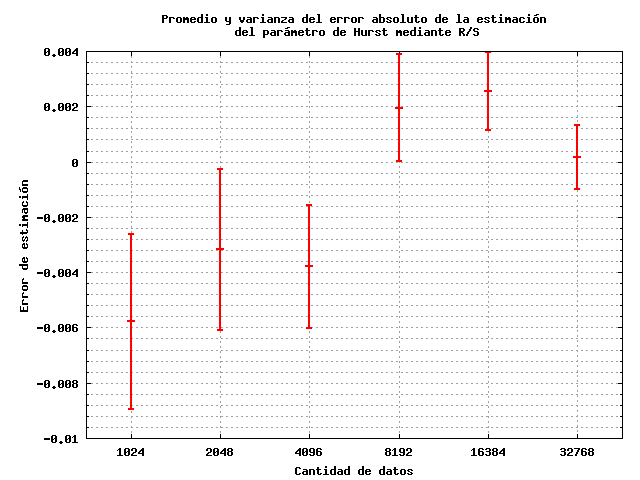
\includegraphics[scale=0.45,type=png,ext=.png,read=.png]{figures/abserror-rs}
\caption{Promedio y varianza del error absoluto de la estimaci'on del par'ametro
de Hurst para el m'etodo estad'istico R/S}
\label{fig:abserrrs}
\end{figure}

\begin{figure}[htb]
\centering
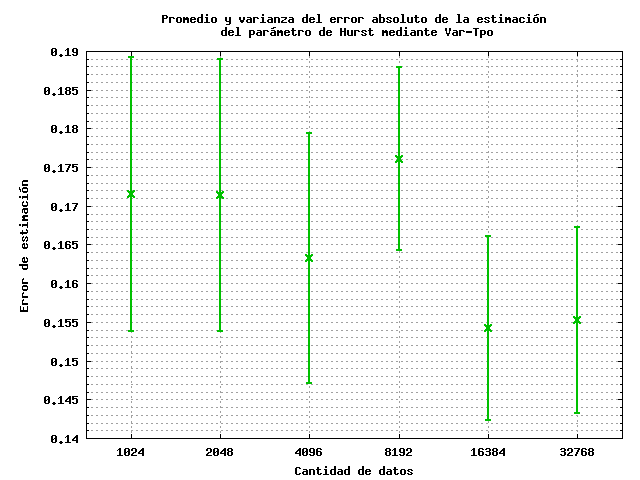
\includegraphics[scale=0.45,type=png,ext=.png,read=.png]{figures/abserror-var}
\caption{Promedio y varianza del error absoluto de la estimaci'on del par'ametro
de Hurst para el m'etodo de gr'aficas de varianza-tiempo}
\label{fig:abserrvar}
\end{figure}

\begin{figure}[htb]
\centering
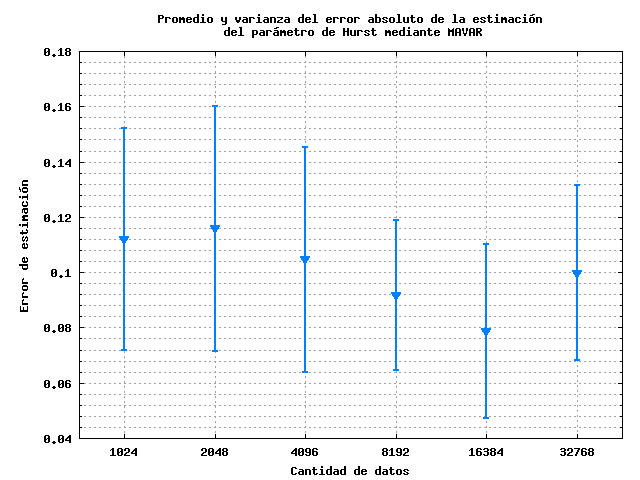
\includegraphics[scale=0.45,type=png,ext=.png,read=.png]{figures/abserror-mavar}
\caption{Promedio y varianza del error absoluto de la estimaci'on del par'ametro
de Hurst para el m'etodo de varianza modificada de Allan}
\label{fig:abserrmavar}
\end{figure}

\clearpage

\begin{figure}[htb]
\centering
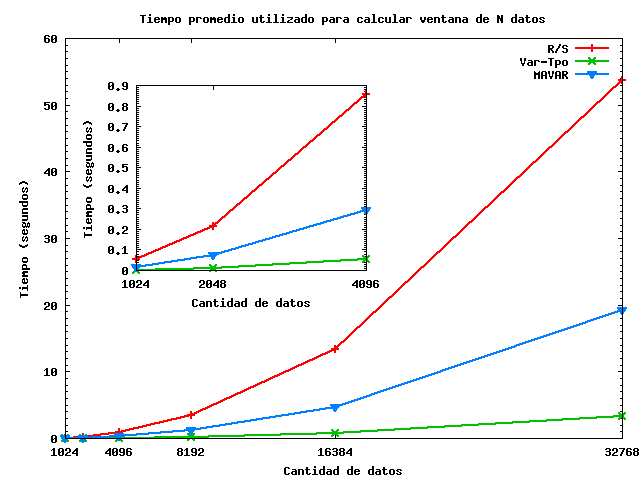
\includegraphics[scale=0.38,type=png,ext=.png,read=.png]{figures/time-n-plot}
\caption{Tiempo promedio utilizado para estimar una ventana de 1024 a 32768
datos para los m'etodos implementados}
\label{fig:tiempoventana}
\end{figure}

Observando las figuras \ref{fig:abserrrs}, \ref{fig:abserrvar} y
\ref{fig:abserrmavar}, lo que se puede evidenciar es que, en general, el
promedio del error absoluto de las estimaciones del par'ametro de Hurst de los
m'etodos mejoran y la varianza disminuye cuando se toman en cuenta un mayor
n'umero de datos para la ventana de estimaci'on. Sin embargo, para los
dos m'etodos que dependen de c'alculos con la varianza el promedio del error 
absoluto de la estimaci'on, incluso con el mayor n'umero de datos es mayor a
$0.1$. El m'etodo del estad'istico R/S es el m'etodo que se comporta mejora 
ya que tiene, en general, un error absoluto muy cerca a $0$ con una varianza
m'inima. 

De acuerdo a \cite{intelligentfuzzy} si queremos analizar los datos en tiempo
real para una red se tendr'ia que hacer una estimaci'on como m'inimo cada
segundo, por lo que una estimaci'on no puede tardar m'as de un segundo en
realizarse. Esto es seriamente limitante ya que cada m'etodo tiene un tiempo de
ejecuci'on muy diferente. Observando la figura \ref{fig:tiempoventana}, con
esta restricci'on la 'unica posibilidad que se tiene es limitar al m'etodo del
estad'istico R/S a $4096$ datos, al m'etodo de gr'aficas varianza-tiempo a
$16834$ datos y al m'etodo de varianza modificada de Allan a $4096$ datos. Dado
que para comparar los m'etodos es importante usar la misma cantidad de datos,
decidimos trabajar con $4096$ datos. El limitar el n'umero de datos va a
afectar la estimaci'on del par'ametro de Hurst directamente como se muestra en
las figuras \ref{fig:abserrrs}, \ref{fig:abserrvar} y \ref{fig:abserrmavar}. 

A pesar de estos problemas, seguimos adelante con el proyecto porque no
queremos una sola estimaci'on puntual y precisa de la traza, sino detectar su
variaci'on, por lo que optamos por un buen balance entre el tiempo de
ejecuci'on y el n'umero de datos a utilizar \cite{intelligentfuzzy}.


